\documentclass[a4paper]{article}

\usepackage[english]{babel}
\usepackage[utf8]{inputenc}
\usepackage{amsfonts}

\usepackage{amsmath}
\usepackage{graphicx}
\usepackage[colorinlistoftodos]{todonotes}

\title{dsPIC33: Exercise}
\author{Pierre Gerard, Julian Schembri, Francois Schiltz}

\setlength{\parindent}{0pt}

\begin{document}
\maketitle

\section{Question 1}

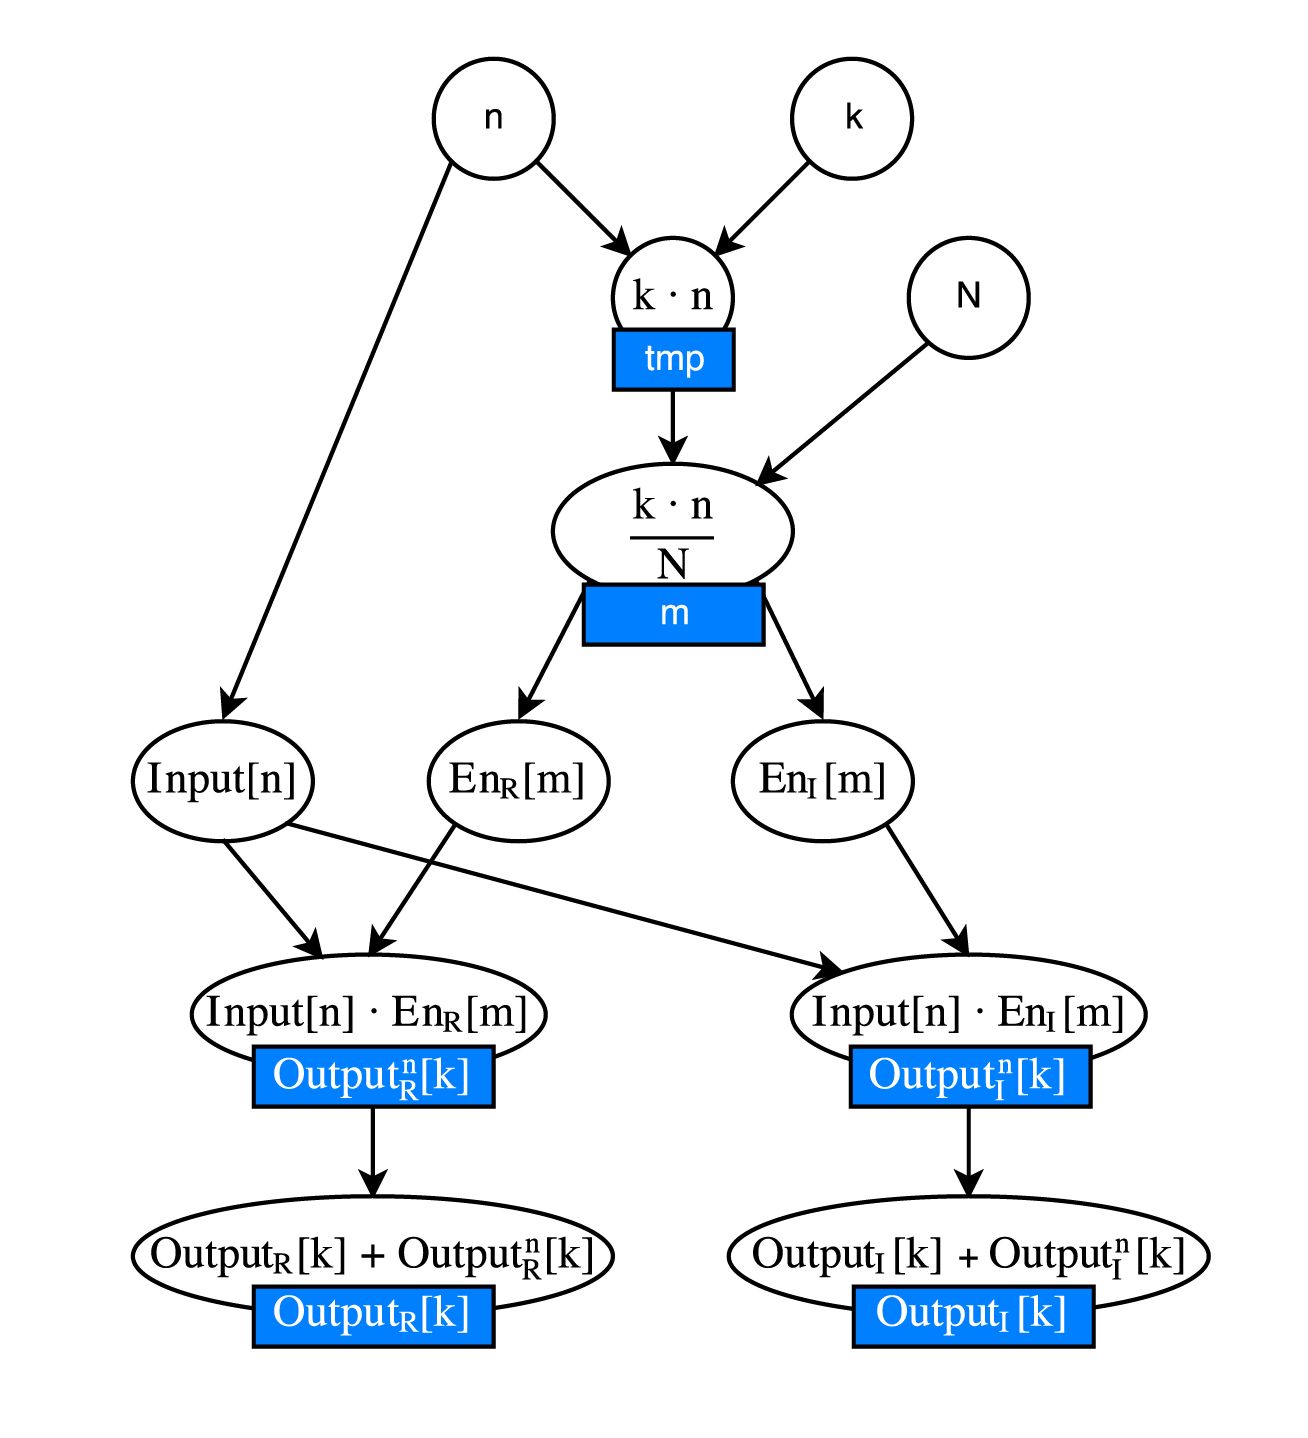
\includegraphics[scale=1]{files/elect-01.png} 

\section{Question 2}

\subsection{Computation of the value m}


\verb|INT16U unsigned16temp;|

\verb|unsigned16temp = (k * n);|

\verb|m = (INT8U) (unsigned16temp / (INT16U) N);|
\\

If we directly do the computation $ m = k*n/N $ we would get a wrong result. In fact the multiplication would be too big and some of the result could overflow and be wrong. To solve that problem, we use a intermediate variable of 16bit to store the result of the multiplication. We then do the division and then cast it back to 8 bits. The cast should be correct because the result of the division (m) should stands on 8 bits if the inputs are correct.

\subsection{Computation of the real part}

\verb|signed16temp_r = (INT16S)input[n] * (INT16S) en_r[m];|
\\
First we cast the two 8 bits fixed point integer to two 16 bits fixed point integer to avoid sign trouble and then do the multiplication as shown in the $example2.c$. We put the result in a 16bits integer so the result would be correct.
\\
\verb|signed8temp = (signed16temp_r+128) >> 8;|
\\
Then we are required to put the result in a 8 bits register, so to get better result we first round it and then do the shift to only keep the most significant bits.
\\
\verb|signed16temp_r = (INT16S) signed8temp + (INT16S) output_r[k];|
\\
At last we add the element of the sum to a temporary 16 bits register. We use a 16 bits temporary variable because the addition of two number on 8 bits could overflow.

\subsection{Computation of the imaginary part}

Actually it is the same as the real part with other variables.

\section{Question 3}

\subsection{Computation of the value m}

\verb|unsigned16temp = (k * n);|

Since we do INT16 = INT8 * INT8 no overflow will occur. Let's take a look at a borderline case :   $ 1111\ 1111 * 1111\ 1111 = 1111\ 1110\ 0000\ 0001 $. There is no information lost so the accuracy is maximum.

\verb|m = (INT8U) (unsigned16temp / (INT16U) N);|

If the input are in there correct range, no overflow will occur because m must be between 0 and 127 included, so it is ok to cast it to a 8 bit integer. Some precision can be lost during the division since the result is a integer all the time. Plus it loose the decimal, so for instance $1.9$ will be $1$ if interpreted as an integer instead of 2 for the nearest integer. Let's take a look at another (non-trivial) borderline case :   $ 0000\ 0001 * 0000\ 0001\ /\ N = 0000\ 0000\ 0000\ 0001 / 128 \Leftrightarrow 0000\ 0000\ 0000\ 0001 \gg 8 = 0000\ 0000 $.

\subsection{Computation of the real part}

\verb|signed16temp_r = (INT16S)input[n] * (INT16S) en_r[m];|
\\
The two 8 bits fixed point integer are cast to two 16 bits fixed point integer so the sign will be correct.
Then since the number stands on 8 bits, it's similar to above for the justification that no overflow happen. Borderline case :   $ 1111\ 1111 * 1111\ 1111 = 1111\ 1110\ 0000\ 0001 $. There is no information lost so the accuracy is maximum.
\\
\verb|signed8temp = (signed16temp_r+128) >> 8;|
\\
Here no overflow could happen. But the last 8 bits are lost.
Since it's signed we lost the precision after the 7th bit of the value.
The accuracy is about $ \frac{1}{2} ^{7}$
\\
\verb|signed16temp_r = (INT16S) signed8temp + signed16temp_r;|
\\
The values signed8temp are between $[-128;127]$. The variable signed16temp\_r is signed 16 bits integer, playing the role of accumulator. It acculates N values where N is equal to 128 which means that the final value of signed16temp\_r is between $[-128*128;127*128]$.
\\
Since we put the result of the addition of two number standing on 8 bits in a 16 bits variable no overflow can happen and the accuracy is maximum. Borderline case : $ 1111\ 1111 + 1111\ 1111 = 0000\ 0001\ 1111\ 1110 $.

\verb|output_r[k] = (INT8S) (signed16temp_r >> 7);|

Output\_r are stored in a signed 8 bits integer that's why the last 7 bits are lost. This time the shift is 7 and not 8 because there is only 128 ($ 2^{7} $) addition.
The accuracy is the same as above, about $ \frac{1}{2} ^{7} $

\subsection{Computation of the imaginary part}

Actually it is the same as the real part with other variables.

\section{Question 4}
The important point is that the buffer can't be modified during the execution of the algorithm. That means that the time between two update should be superior to the execution time of the algorithm.

\begin{center}
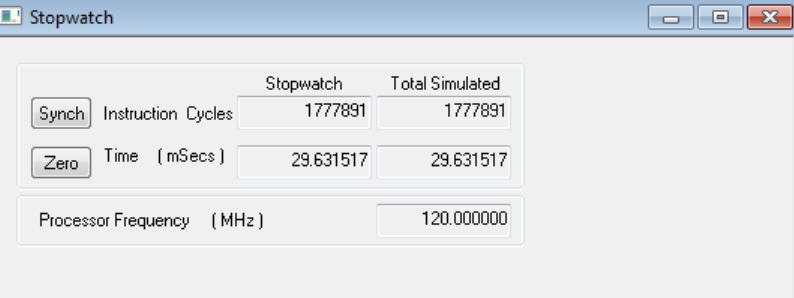
\includegraphics[scale=0.5]{files/stopwatch.png} 
\end{center}

The algorithm need 1 777 891 cycles to run. We used the debugger to get that value, which is more precise than a approximation using the sum of individual operation done in the lab.

The time for a cycle depends of the frequency of the internal clock.

If we suppose that the frequency of the microcontroller is 120MHZ as suggested by the debugger, a cycle would take $ \frac{2}{120 * 10^{6} }$. The 2 stands there because on the pic33 it takes 2 clock cycle for an instruction cycle.

So the maximum time between two buffer update is $ \frac{2}{120 * 10^{6} } * 1 777 891 =  29,63 ms $

And the maximum frequency for buffer updtae is about 33.75 Hz. 

\end{document}